\subsection{Task 6: lattice translation}

A simple (though inefficient) way to translate a source sentence in non-monotone order would be to enumerate all alternative permutations and translate them individually.
Then, with some appropriate decision rule, we select the final translation.
Besides inefficient, some decision rules can only be defined in the combined space of translations.

Now that the permutations have been efficiently represented using transducers, translating these permutations is no different from translating a trivial linear finite-state transducer.
That is right, all it takes is a composition between the input lattice and the phrase-table transducer.
Figure \ref{fig:non-mono} illustrates the composition between the permutation lattice in Figure \ref{fig:permutations} and the phrase table in Figure \ref{fig:rules}.

\begin{figure}[h]\centering
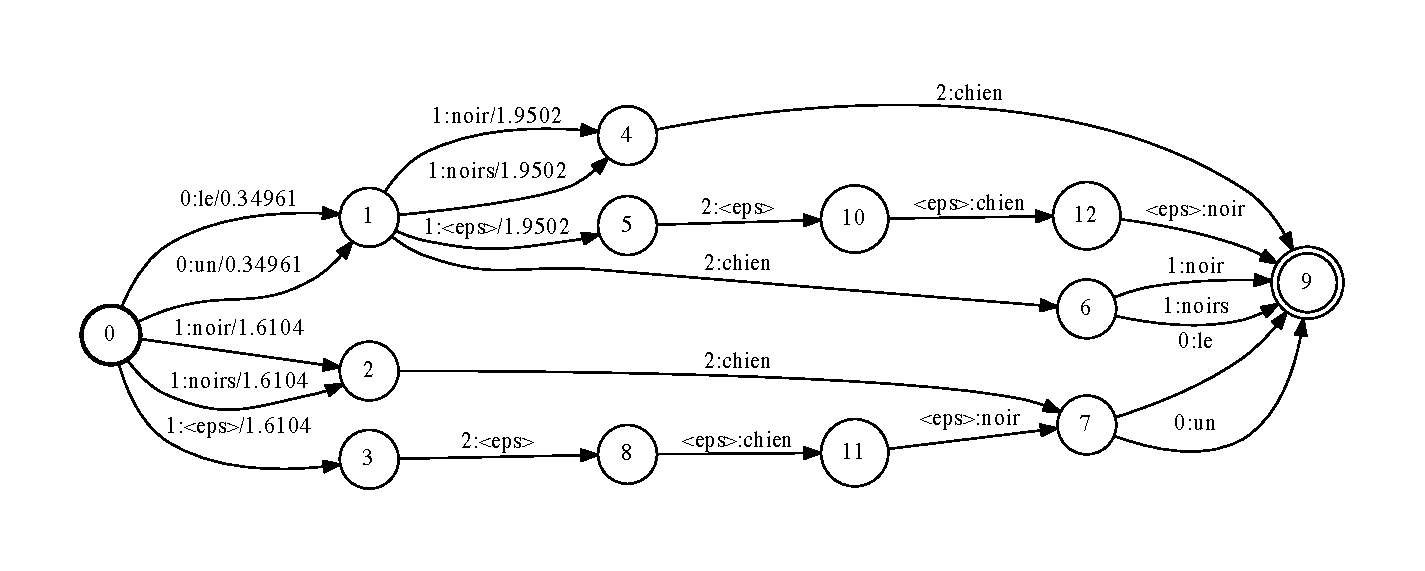
\includegraphics[scale=0.5]{lattice-nonmonotone.pdf}
\caption{\label{fig:non-mono}Translation derivations for permutations of the input.}
\end{figure}


Because we have changed the space of translations of our model (by including translations of permutations of the input), and because we have added a new feature to the linear combination (i.e. \texttt{LatticeCost}), it makes sense to re-estimate the parameters of the linear model.
You will not need to do it yourself,\footnote{But wait for project 3 ;)} as I have already provided you with \texttt{weights.lattice}.
You will need, however, to recompile your phrase tables so that they are weighted by the correct linear model.
Table \ref{tab:task6} summarises the task. 




\begin{table}[h]\centering
\begin{tabular}{l p{12cm}}
\textsc{Task}   &  translate permutation lattices\\
\textsc{Input}  &  one permutation lattice per sentence and a recompiled weighted transducer per phrase table\\
\textsc{Output} &  a weighted set of translation derivations per sentence\\
                &  100-best paths from each transducer \\
                & \emph{best-derivation} and \emph{best-translation} decision rules\\
\textsc{Submit} & \texttt{lattice.100best.}$n$: 100-best derivations from each transducer in text format with alignments\\
                & \texttt{lattice.der} and \texttt{lattice.trans} \\  
\textsc{Report} & BLEU score for each decision rule using references in \texttt{dev.ja}\\
\end{tabular}
\caption{\label{tab:task6}Task 6 summarised}
\end{table}
